\chapter{Introduction}

\label{ch:intro}

The Mu2e Raw Data Mover (RDM) System is an element of Mu2e Data Processing
and Computing (DPC), an L2 project within Mu2e Experiment Operations Plan.
\fixme{cite the EOP}
Its purpose is to move data
that is produced by the online system to long term storage;
for most data, the long term storage will be files on tape
but, for some data, it will be in one of the offline databases.
Some data may also reside transiently in disk files so that
it is readily avaialble for the follow-on data processing steps.

Other functions of the RDM include:
\begin{enumerate}
\item Updating the file catalog to include meta-data and file location(s).
\item Any splitting/joining or other reshaping of files that is needed to match the needs of downstream processing.
\item Managing the free space in the online disk buffer
\item Copy/mirror subsets of the online databases to the offline databases
\end{enumerate}

It is expected that the offline data processing workflows will be driven by updates to the file catalog;
so the RDM does not need other hooks into those workflows.

The operation and maintenance of the network between the Mu2e Hall and the computer center
is the responsibility of the Fermilab Core Computing Division (CCD).
The DPS has the responsibility to be the interface between Mu2e and CCD regarding this network.
Details of this responsbility are in Section~\fixme{reference the appropriate section}.

In early planning for the Mu2e DPC, what is now called the RMD was called the Data Logging System.
However that name is too class to two related concepts in the online world:
the {\tt artdaq} DataLogger processes that run on the Data Logger nodes at the end of the TDAQ
processing change.  The name was changed to RDM to avoid confusion.

\section{Conventions Used in this Document}

In this document the word ``computer center'' is used as a collective noun for the
Feynman Computing Center (FCC) and the Grid Computing Center (GCC).
When it is important to distinguish the two, one of the two will be named explicitly.



\section{If you are an HEP Software expert...}

Section 2 of chapter 1

\chapter{The Next Chapter}
\label{ch:next_chapter}

This is chapter 2 and refers to Figure~\ref{fig:interfaceTDAQ}

\begin{figure}[tbp]
\centering
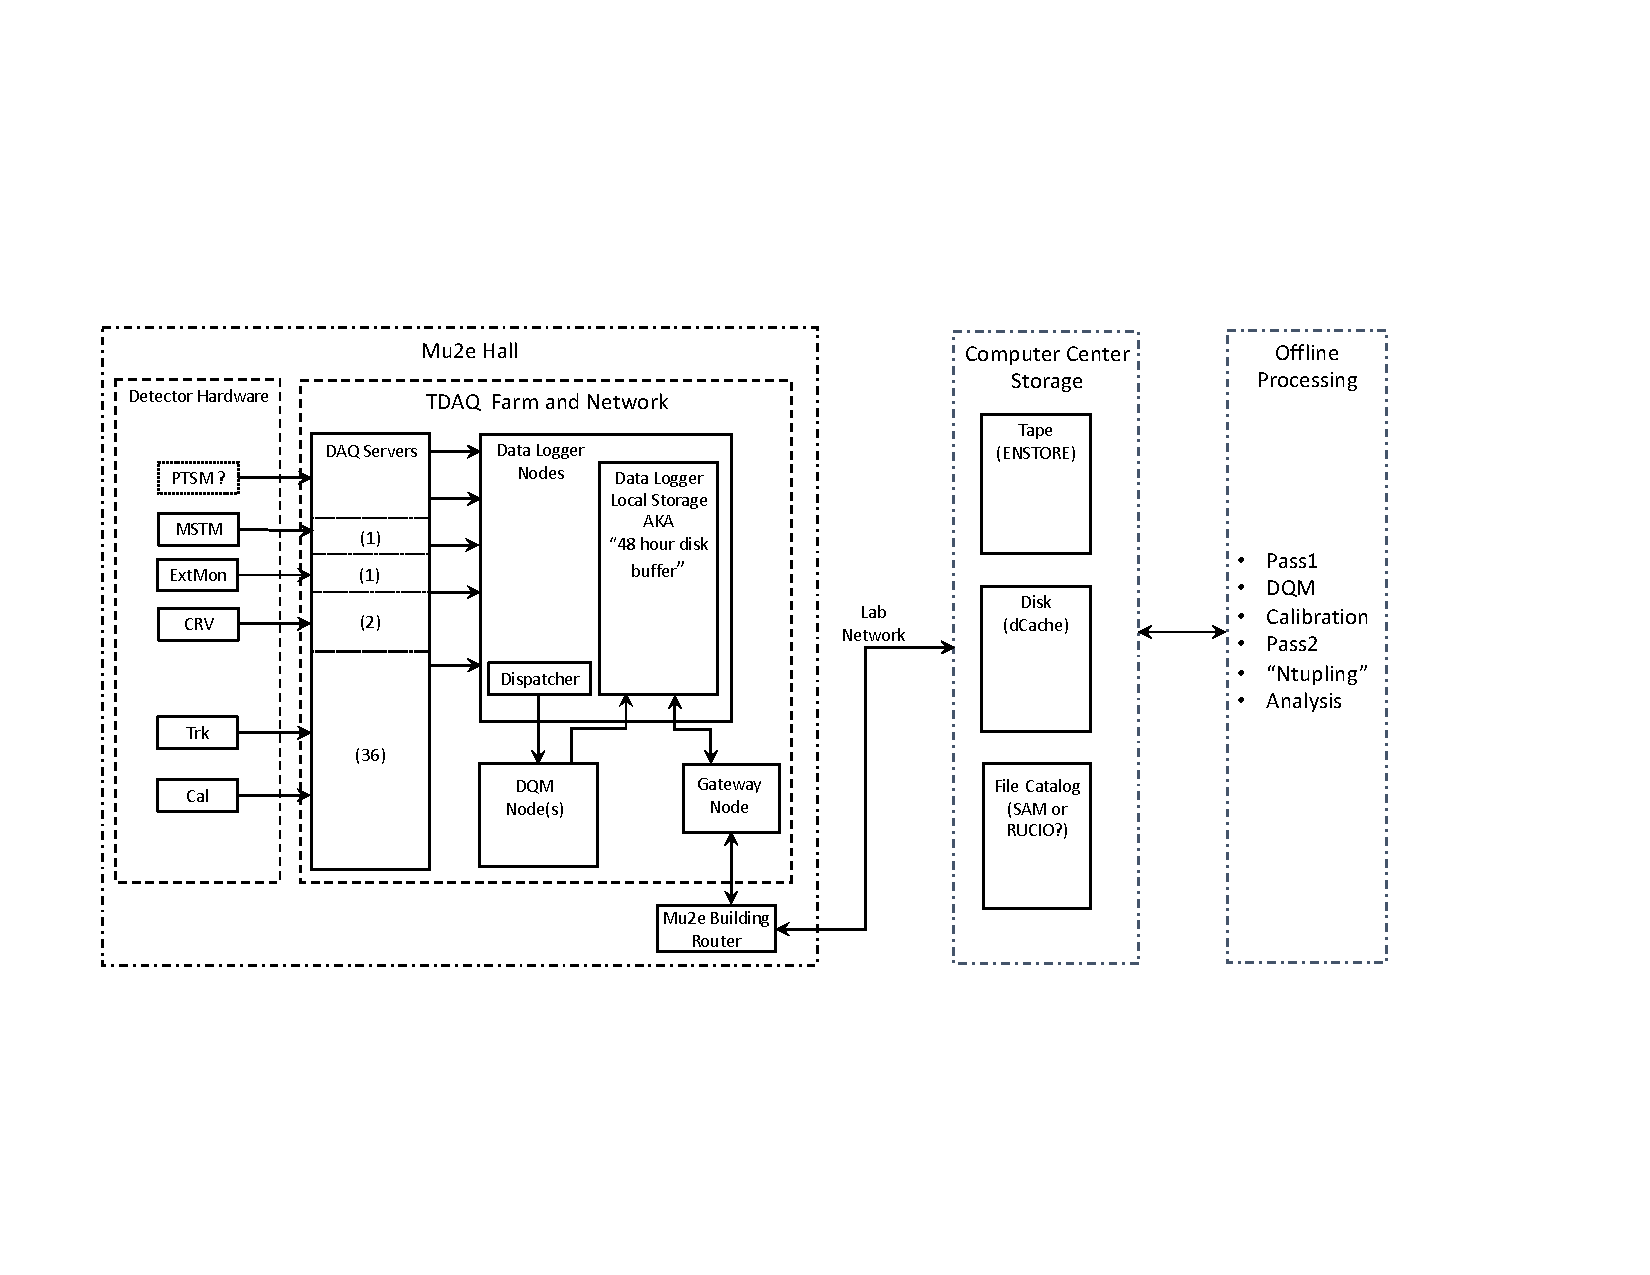
\includegraphics[width=0.9\textwidth]{figures/interface_with_TDAQ.pdf}
\caption{The interface with the TDAQ System}
\label{fig:interfaceTDAQ}
\end{figure}


\section{If you are new to HEP Software...}

Section 1 of chapter 2


\section{If you are an HEP Software expert...}

Section 2 of chapter 2


% Keep sections under development
\IfStrEq{\ISDRAFT}{YES}{

\chapter{A Chapter under development}
\label{ch:under_development}

This is a chapter still under development

\section{If you are new to HEP Software...}

Section 1 of a chapter still under development


\section{If you are an HEP Software expert...}

Section 2 of a chapter still under development

} % end `ISDRAFT = YES'


\appendix

\chapter{SubRuns}
\label{ch:app_Subruns}

This appendix has information about subruns

\section{If you are new to HEP Software...}

Section 1 of the appendix on subruns that refers to Table~\ref{tab:clhep:functions}.
\begin{table}
\begin{center}
\caption[Selected member functions of {\tt CLHEP::Hep3Vector}]{Selected member functions of {\tt CLHEP::Hep3Vector}.}
\label{tab:clhep:functions}
\begin{tabular}{lll}\hline
  {\cppfcl a = u.cosTheta();}  & {\cppfcl double cosTheta() const;} & $\cos\theta$\\
  {\cppfcl a = u.cos2Theta();} & {\cppfcl double cos2Theta() const;} & $\cos^2\theta$\\
  {\cppfcl v = u.unit();}      & {\cppfcl Hep3Vector unit() const;} & A unit vector in the direction of {\cppfcl u} \\ \hline
  \end{tabular}
\end{center}
\end{table}


\section{If you are an HEP Software expert...}

Section 2 of the appendix on subruns.

\chapter{DQM Data}
\label{ch:DQM data}

This appendix has information about subruns

\section{If you are new to HEP Software...}

Section 1 of the appendix on subruns.


\section{If you are an HEP Software expert...}

Section 2 of the appendix on subruns.

\cleardoublepage
\printindex

